%
% Clases de módulo de BPS.
% Análisis y diseño de programa tokenizador, reporte técnico.
%
% Proyecto Lovelace.
%

\subsection{Clases de \texorpdfstring{\acrshort{gl:bps}}{BPS}}

Primero, se tiene que mencionar que a pesar de que \gls{gl:bps} puede verse como
una versión más específica de \gls{gl:ffx}, esta clase no se realizó de forma
directa a partir de la clase de la red Feistel.

A \gls{gl:bps} se le puede considerar como un modo de operación que usa un
cifrado interno BC, que a su vez usa un cifrado de ronda, situación por la que
\gls{gl:bps} es una clase que implementa el modo de operación descrito en
\ref{sec:bps_modo_operacion}, que utiliza la clase BC, cuyo funcionamiento se
describe en~\ref{sec:bps_cifrador_interno_bc}, el cual se puede resumir como
una red Feistel que opera sobre cadenas construidas a partir de cualquier
alfabeto, en vez de sobre cadenas binarias.

En cuanto al cifrado de ronda, esta clase se construyó usando la librería de
Cripto++, dando la posibilidad de usar \gls{gl:aes} o \gls{gl:des}.

% ¿Triple DES, no?

El diagrama de clases del módulo de \gls{gl:bps}, sin contemplar las clases del
paquete de utilidades, se muestra en la figura~\ref{diagrama_clases_bps}.

\begin{sidewaysfigure}
  \begin{center}
    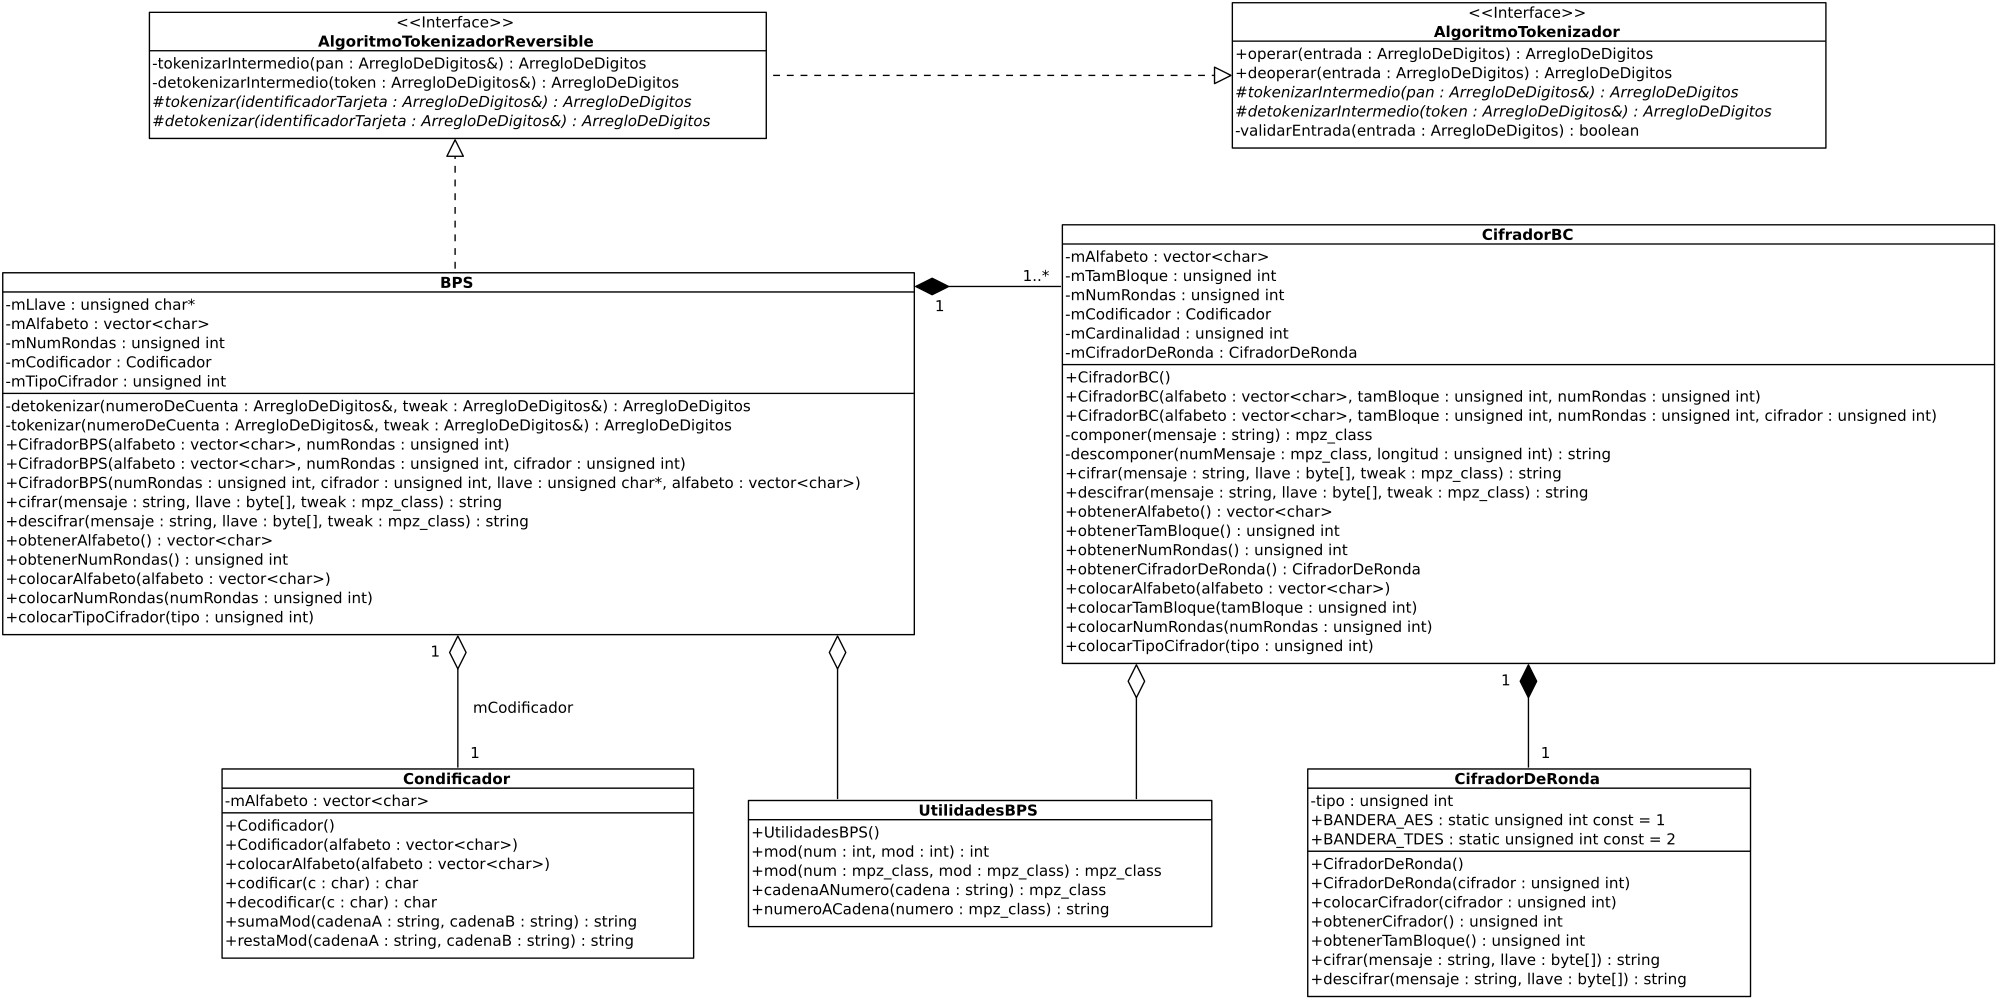
\includegraphics[width=1.0\linewidth]{diagramas/bps.png}
    \caption{Diagrama de clases de módulo de \gls{gl:bps}.}
    \label{diagrama_clases_bps}
  \end{center}
\end{sidewaysfigure}
